\documentclass{article}

% if you need to pass options to natbib, use, e.g.:
% \PassOptionsToPackage{numbers, compress}{natbib}
% before loading nips_2017
%
% to avoid loading the natbib package, add option nonatbib:
% \usepackage[nonatbib]{nips_2017}

\usepackage[final]{nips_2017}

% to compile a camera-ready version, add the [final] option, e.g.:
% \usepackage[final]{nips_2017}

\usepackage{graphicx}
\usepackage[utf8]{inputenc} % allow utf-8 input
\usepackage[T1]{fontenc}    % use 8-bit T1 fonts
\usepackage{hyperref}       % hyperlinks
\usepackage{url}            % simple URL typesetting
\usepackage{booktabs}       % professional-quality tables
\usepackage{amsfonts}       % blackboard math symbols
\usepackage{nicefrac}       % compact symbols for 1/2, etc.
\usepackage{microtype}      % microtypography
\usepackage{amsmath}
\usepackage[linesnumbered,ruled]{algorithm2e}
\title{Edge Machine Learning for Resource-constrained\\IoT Devices}

% The \author macro works with any number of authors. There are two
% commands used to separate the names and addresses of multiple
% authors: \And and \AND.
%
% Using \And between authors leaves it to LaTeX to determine where to
% break the lines. Using \AND forces a line break at that point. So,
% if LaTeX puts 3 of 4 authors names on the first line, and the last
% on the second line, try using \AND instead of \And before the third
% author name.

\author{
  Haocheng Fang \\
  Carnegie Mellon University \\
  \texttt{hfang@andrew.cmu.edu} \\
  \And
  Yichen Ruan \\
  Carnegie Mellon University \\
  \texttt{yichenr@andrew.cmu.edu} \\
  \And
  Jinhang Zuo \\
  Carnegie Mellon University \\
  \texttt{jzuo@andrew.cmu.edu} \\
  %% examples of more authors
  %% \AND
  %% Coauthor \\
  %% Affiliation \\
  %% Address \\
  %% \texttt{email} \\
  %% \And
  %% Coauthor \\
  %% Affiliation \\
  %% Address \\
  %% \texttt{email} \\
  %% \And
  %% Coauthor \\
  %% Affiliation \\
  %% Address \\
  %% \texttt{email} \\
}

\begin{document}
% \nipsfinalcopy is no longer used

\maketitle
\section{Introduction}


Edge computing, also known as fog computing, aims to fully utilize the computing power of resource-constrained devices that are physically close to end users. Compared to traditional cloud services, edge computing promises light weight solutions for budget-constrained and latency-sensitive computing tasks. The deployment of machine learning algorithms on the edge architecture is appealing and has great practical value. For applications like real-time anomaly detection and offline identity verification, edge machine learning avoids the latency of data transmission, and often offers strong privacy protection as well as security guarantee.

A straightforward idea to deploy machine learning on edge devices is using distributed machine learning algorithms. However, these existing methods typically fail to work due to the resource-constrained nature of edge IoT devices. There are thus emerging demands for novel models and algorithms. In this project, we propose a tree-based classification model for multiple resource-constrained IoT devices. It utilizes prior knowledge (e.g., hierarchy in Figure 1) to build a large classification tree with identical hierarchy to the prior knowledge at first, then prunes the tree node by node while minimizing accuracy loss. Pruning stops when the number of classifier in the classification tree is equal to the number of available IoT devices and we reach an optimal state where the final model can fit on the limited number of devices while having minimal accuracy loss.

There are two main advantages of this classification model. The first one is that we have very low requirements on the computing power of each node. We can combine numerous resource-constrained devices to obtain a classification model with high accuracy that is otherwise not possible on such devices. The model can also scale up whenever new nodes are added and improve the overall accuracy. The second advantage is that in our tree-based classification model, each node only propagates the data to the lower branch with the highest probability. Therefore, the utilization of each node is very low and this allows for high levels of parallelization and increased throughput when working on large number of images. 

For our experiments, we plan to use Neural Networks(NNs) to solve image classification tasks. Therefore, instead of running a huge network that classifies the entire dataset, we can run multiple small networks that distinguish specific elements. For example, if we are to classify between thousands of species of animals, we can first use prior knowledge about the hierarchy of the animals to create nodes that classify between different species and then create different nodes that classify between various breeds under a specific species. The entire framework will look like a tree with each node being a small NN running on an IoT device. The main challenge of the project is to create an optimal model that best splits the data while being able to fit the NNs on each node. For experiments, we will deploy the models onto Raspberry Pi’s for image classification on the CIFAR-100 dataset.

\begin{figure}[ht]
  \centering
  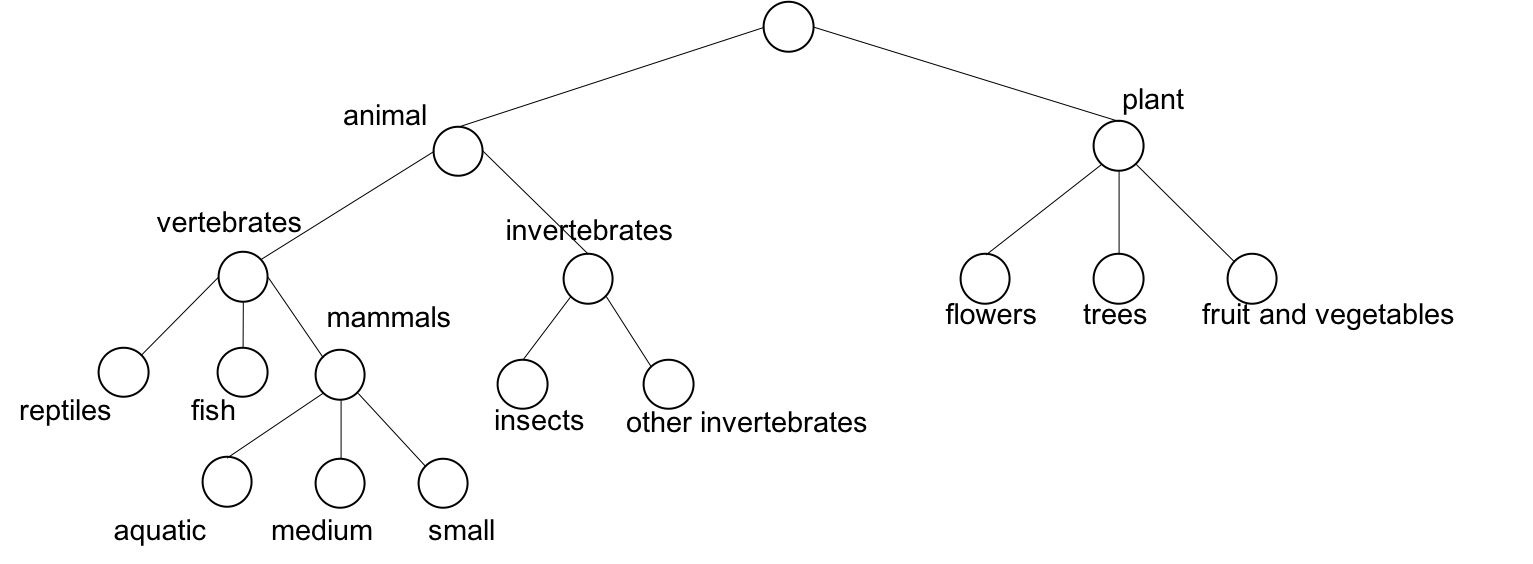
\includegraphics[width=0.8\textwidth]{cifar100.png}
%   \fbox{\rule[-.5cm]{0cm}{4cm}{fig1.jpg} \rule[-.5cm]{4cm}{0cm}}
  \caption{Hierarchy of CIFAR-100 dataset}
\end{figure}

\section{Related Work}
While machine learning becomes essential for lots of IoT applications, most of IoT devices make predictions via sending their measurement data to centralized clouds [1, 2]. Compared to centralized prediction, having edge devices make predictions locally avoids the latency of data transmission, and offers strong privacy protection [4]. One way to deploy machine learning onto multiple edge devices is distributed machine learning [5 - 8]. However, existing distributed machine learning, which aims to enable large-scale ML task, does not consider memory and computing constraints on the edge devices, thus cannot be used directly by edge devices. 

There are many adaptive systems considering resource-constrained prediction, which ensure overall accuracy under budget constraints [9, 10]. Nan \& Saligrama [11] propose an adaptive approximation approach for test-time resource-constrained prediction motivated by IoT. In [12], a random forest is pruned to optimize expected feature cost and accuracy for resource-constrained prediction. 

Another set of related work designs resource-efficient small models which can run on IoT devices.  Kumar et al. [4] develop a novel tree-based algorithm for efficient prediction on IoT devices. Gupta et al. [13] proposes ProtoNN, a novel kNN based algorithm for tiny resource-constrained devices to solve supervised learning problems. The Sparse Multiprototype Linear Learner (SMaLL) algorithm in [14] is used for training small resource-constrained predictors.

\section{Method}
The basic idea of our method is to group classes into some superclasses. And organize those superclasses as a hierarchical tree-structure. Then we assign one edge device to each vertex of the tree. The expectation is to reduce the complexity of models on each node, and increase the prediction accuracy.  What is more, instead of building a classification model over the whole dataset, each individual edge node now works on a single group that contains only a subset of the total data. In that way, we can reduce the storage and communication overhead of the whole network.

For example, suppose we want to classify human images into 4 categories: women, girls, men and boys. And assume we only have 3 edge devices available. We can create a ``females" superclass by grouping women and girls. Similarly, we group men and boys as a ``males" superclass. Then, we can assign a edge device to determine if the image is female or male; assign one device to classify women and girls out of females; and use the last device for men and boys. Upon a request, the first node that works as the root of the tree will predict if the observation is female or male. Once it gets the result, it will forward the request to nodes in the next level. Eventually, the leave nodes will yield the final result. It is worthnoting that the way classes are grouped is generally not unique. For example, we can also merge women and men as an ``adult" superclass; merge girls and boys as an ``children" superclass. Other combination is also possible if that yields good classifiers.

\begin{figure}[ht]
  \centering
  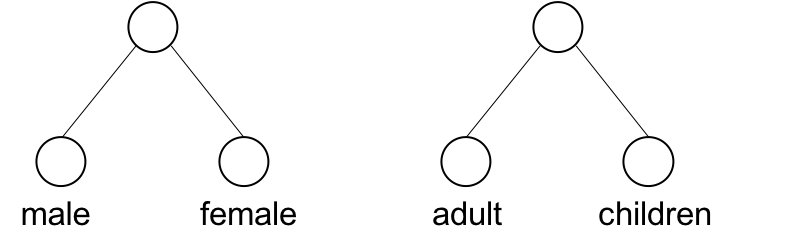
\includegraphics[width=0.6\textwidth]{4_class.png}
%   \fbox{\rule[-.5cm]{0cm}{4cm}{fig1.jpg} \rule[-.5cm]{4cm}{0cm}}
  \caption{Two possible topology for 4 classes: women, girls, men and boys}
\end{figure}

As is discussed above, the topology of the groups can be organized as a tree (call it a t-Tree). Each edge node is associated with a t-Tree node, which trains a machine learning model to classify its children. On prediction, a query starts from the root, and goes all the way to the leaves. The prediction result is the class reported by the last t-Tree node on the path. 

Algorithm \ref{ag:prediction} illustrates the process of prediction an observation. The complexity of the algorithm is bounded by the height of the t-Tree, which is roughly $O(\log(L))$, where $L$ is the total number of classes. Though the prediction accuracy of each node is increased because of fewer classes, the error is propagating in a tree structure. For the purpose of reducing error and pipelining queries, we want the upper level nodes to have higher accuracy and shorter runtime. Moreover, we want the tree to be shorter such that the error does not accumulate alongside a long path.

\begin{algorithm}[H] \label{ag:prediction}
    \SetKwInOut{Input}{Input}
    \SetKwInOut{Output}{Output}

    \underline{function Predict $(T, X)$}\;
    \Input{A t-Tree node $T$; A sample $X$}
    \Output{A class label}
    \eIf{$T$ is leave}
      {
        return $T$.classifier.predict($X$)
      }
      {
        id = $T$.classifier.predict($X$)\\
        $T'$ = $T$.children(id)\\
        return Predict($T',X$)
      }
    \caption{Prediction Algorithm}
\end{algorithm}

Generally, if we have $k$ edge devices and $L$ classes, our purpose is to find the optimal tree structure that maximizes the average prediction score. The average prediction score of a sub-tree rooted at $T$ is defined recursively as follows. We define the score of whole system as the score of the root node.
\begin{equation}\label{eq:score}
\text{Score}(T)=\left\{
                \begin{array}{ll}
                  T.\text{accuracy, if $T$ is leave}\\
                  T.\text{accuracy}\times \frac{1}{|T|}\sum_{C\in T.\text{children}}|C|\text{Score}(C), \text{otherwise}
                \end{array}
              \right.
\end{equation}
where $T.\text{accuracy}$ is the training accuracy of the classifier inside $T$, which could be accuracy on the training data or that on the hold-out data. $|T|$ is the number of samples of node $T$, which is the sum of that of its children. The definition is simply the accuracy of the root, multiplied by the number-of-samples-weighted average accuracy of its children. An possible alternative is instead of the average performance, we define the score as per the worst case. 
\begin{equation} \label{eq:score2}
\text{Score}(T) = \min_\Gamma{\prod_{C\in \Gamma}C.\text{accuracy}}
\end{equation}
where $\Gamma$ is a path from $T$ to some leave node. We use the first definition in this project because we are more focusing on the average performance of the system. The second definition can be a good reference if the requests are highly skewed or one has strict requirements on the minimal accuracy guarantee.

Ideally, we want to find a t-Tree structure that maximizes the average accuracy. The problem is however very hard considering the possibilities of tree topology. Without a constraint on the tree structure, the number of combinations can be exponential with respect to number of classes $L$. Our idea is thus to limit the topology a t-Tree can take, thus pruning the searching space. We will discuss two pruning algorithms in Section \ref{ss:baseline} and
\ref{ss:texonomy}.

We generally do not set limitations for the types and complexities of individual classification models. It is possible to use totally different models for different nodes. In the case the same model is used across the tree, one can still set different values for the tuning variables of different nodes. However, for efficiency consideration, it is wise to constraint the choice to a small set of models.

\subsection{A baseline algorithm} \label{ss:baseline}
A naive idea is to constrain the topology as a 2-layer tree. Algorithm \ref{ag:baseline} yields a 2-layer t-Tree with precisely $k$ nodes. The initialization needs to train  $\binom{L}{2}$ models, which takes $O(L^2)$ time. For each iteration in the while loop, the algorithm compares all pairs of leaves, which again takes $O(L^2)$ time. Upon merging a pair of nodes, we need to train two classification models, one for the merged node, one for the parent (i.e. the root node). Other nodes' accuracy are unchanged. There are $L/2-k$ iterations, thus the complexity is $O(L^3)$ times the runtime for training, which could also be quite huge. 

Although the algorithm is extremely slow, it doesn't rely on any prior knowledge of the categories. The two-layer structure means there are precisely two hops before the final prediction result is generated. Thus, the error does not accumulate that much as in a deep-tree. Also, the runtime of the system is more predictable, which is an important property for a stable and reliable system.

\begin{algorithm}[H]\label{ag:baseline}
    \SetKwInOut{Input}{Input}
    \SetKwInOut{Output}{Output}
    \SetKwRepeat{Do}{do}{while}

    \underline{function Build-Tree-Baseline $(k, data, class)$}\;
    \Input{Number of edge nodes $k$; $n$ observations $data$; $L$ class labels $class$}
    \Output{A t-Tree $T$}
    For each pair of classes $(c1,c2)$ in $class$, create a node that classifies $c1$ and $c2$ over $data[\text{label}=c1]+data[\text{label}=c2]$, calculate the training accuracy.\\
    Find the $L/2$ groups that cover all the classes and have the highest accuracy, create a leave node for each of them. Add them to a set $S$.\\
    Create a root node $T$ that points to all nodes in $S$. Train $T$ over the $L/2$ super-classes.\\
    Creates an empty hash table $H$.
    
    \While{len(S) $> k - 1$}
      {
        For each pair $(l_1,l_2)$ in $S$, if it is not in $H$, try merge them, calculate the average score for the new tree structure as in Eq. \ref{eq:score}. Put the result (call it merging score) into $H$ using $(l_1,l_2)$ as key.\\
        Find in $H$ the pair $(l_1^*,l_2^*)$ with the highest merging score.\\
        Merge $(l_1^*,l_2^*)$ to create and train a new node $p$ on corresponding entries of $data$.\\
        $T.\text{children.remove}([l_1^*,l_2^*])$\\ $T.\text{children.add}(p)$\\
        Re-train the root $T$ over $data$ and the new super-classes.\\
        $S.\text{remove}([l_1^*,l_2^*])$\\
        $H.\text{remove}((l_1^*,l_2^*))$
      }
    return $T$\;
    \caption{Baseline Algorithm}
\end{algorithm}

Fig. \ref{fig:example_baseline} shows an example with $k=3, L=6$. It takes $\binom{6}{2}=15$ comparisons to go from state I to II. Three superclasses are generated after the first merging. A root node is created to classify over the 3 groups. To further reduce the number of nodes to 
$k=3$, one more step is required. This takes another $\binom{3}{2}=3$ comparisons. Finally, the ``bird+flower" node and the ``tree+fruit" node is merged. The resulting tree in state III has precisely 3 nodes.


\begin{figure}[ht]\label{fig:example_baseline}
  \centering
  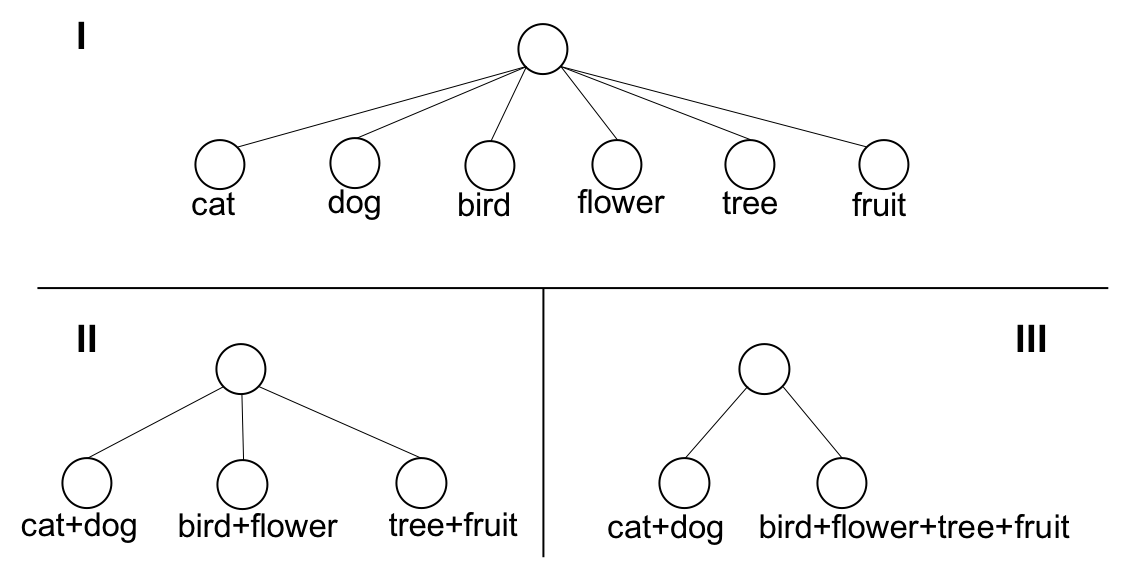
\includegraphics[width=0.7\textwidth]{6_class.png}
%   \fbox{\rule[-.5cm]{0cm}{4cm}{fig1.jpg} \rule[-.5cm]{4cm}{0cm}}
  \caption{Apply the baseline algorithm to a 6-class example. I: initial layout. II: after initialization. III: after first iteration, also the final structure.}
\end{figure}

\subsection{Taxonomy based algorithm}\label{ss:texonomy}
The baseline algorithm is straightforward yet very inefficient. In this section, we will propose a new algorithm that utilizes taxonomy as prior knowledge. 

In fact, for most classification problems, the class labels are highly hierarchical. For example, biology taxonomy classifies species with a 9-layer tree: life, domain, kingdom, phylum, class, order, family, genus and species. So instead of building everything from scratch, we can create a t-Tree by modifying the ``taxonomy tree". We argue that this method is reasonable because: 1) Taxonomy is a science that groups together classes with similar properties, which is usually what machine learning algorithms do; 2) There are many existing algorithms specifically designed for some groups in the taxonomy, which can be reused.

\begin{algorithm}[H]\label{ag:taxonomy}
    \SetKwInOut{Input}{Input}
    \SetKwInOut{Output}{Output}
    \SetKwRepeat{Do}{do}{while}

    \underline{function Build-Tree-Taxonomy $(K, data, G)$}\;
    \Input{Number of edge nodes $K$; $n$ observations $data$; Pre-built taxonomy tree $G$}
    \Output{A tree structure $T$ with at most $K$ nodes.}
    $T$ = $G$ \\
    \While{$|T| > k$}
      {
        For each new pair $(l_1,l_2)$ with the same parent, try merge them. \\
        Compute the change of the average score. Store the result into some global table.\\
        Find in the table the pair $(l_1^*,l_2^*)$ with the highest merging score.\\
        Merge $(l_1^*,l_2^*)$, insert the new node $l_{new}$ under $p = l_1^*.parent$.\\
        \If{$p$ has only one child}
        {
            Replace $p$ with $l_{new}$
        }
      }
    return $T$
    \caption{Taxonomy based Algorithm}
\end{algorithm}

In algorithm \ref{ag:taxonomy}, a node can only merge with its leave-siblings. In the case when a new node becomes an only child, its parent is replaced by the new node. This is the only situation where the height of the tree decreases. After each iteration, the number of nodes will decrease by at least one. The algorithm will therefore stop after a finite number of iterations. The exact decrease of the computation time is depending on the structure of the taxonomy tree. Generally, the runtime gets smaller as the tree has more branches. Assume the tree is balanced, and suppose the $L$ classes are evenly divided into $L/\epsilon$ groups, the runtime for each iteration is at most $O(\frac{L}{\epsilon}\binom{\epsilon}{2})$, which is greatly less than the baseline algorithm situation $O(\binom{L}{2})$.

Fig. \ref{fig:example_taxonomy} applies the taxonomy based algorithm to the same example as in section \ref{ss:baseline}. We need to compare $2\times\binom{3}{2}=6$ pairs from state I to state II, and another $2\times \binom{2}{2}=2$ pairs from state II to state II. The total number of comparisons is 8, which is a huge decrease compared to the 18 comparisons taken by the baseline case.

\begin{figure}[ht]\label{fig:example_taxonomy}
  \centering
  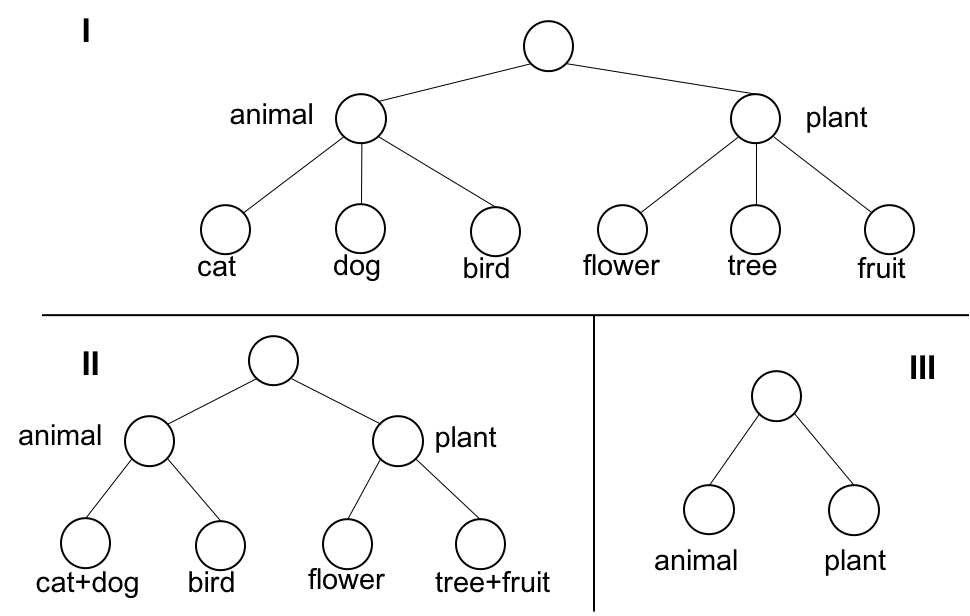
\includegraphics[width=0.7\textwidth]{6_class2.png}
%   \fbox{\rule[-.5cm]{0cm}{4cm}{fig1.jpg} \rule[-.5cm]{4cm}{0cm}}
  \caption{Apply the taxonomy based algorithm to a 6-class example. I: initial layout. II: after first two merge. III. after all level-two nodes are merged, also the final structure.}
\end{figure}

\section{Dataset \& Preliminary Results}
\subsection{Dataset}
CIFAR-100:\\
It contains 100 classes with 600 32x32 colour images each. The 100 classes are then grouped into 20 superclasses. 
We chose this dataset because there exists a hierarchy of all the classes and can serve as prior knowledge to our model. 
We do not need to pre-process the images but we might need to identify a hierarchical structure different from the existing “superclass-subclass” structure. The inputs are the images as numpy arrays and the outputs are the classification results of both the class and superclass(es). 

\subsection{Preliminary Results}
We run our taxonomy based algorithm on part of the CIFAR-100 dataset (as shown in figure 1). We assume that there are 12 available IoT devices. The new taxonomy-based tree is shown in figure 2. Each node in the tree represents a classifier. Table 1 shows the classification accuracy of each node. We can see for some nodes (e.g., mammals), the accuracy is too low. One reason might be that we only use a very small Neural Network (around 10 neurons) on each node. We will try to use larger Neural Network to achieve higher accuracy, while considering the resource constraints on each node.

\begin{figure}[ht]
  \centering
  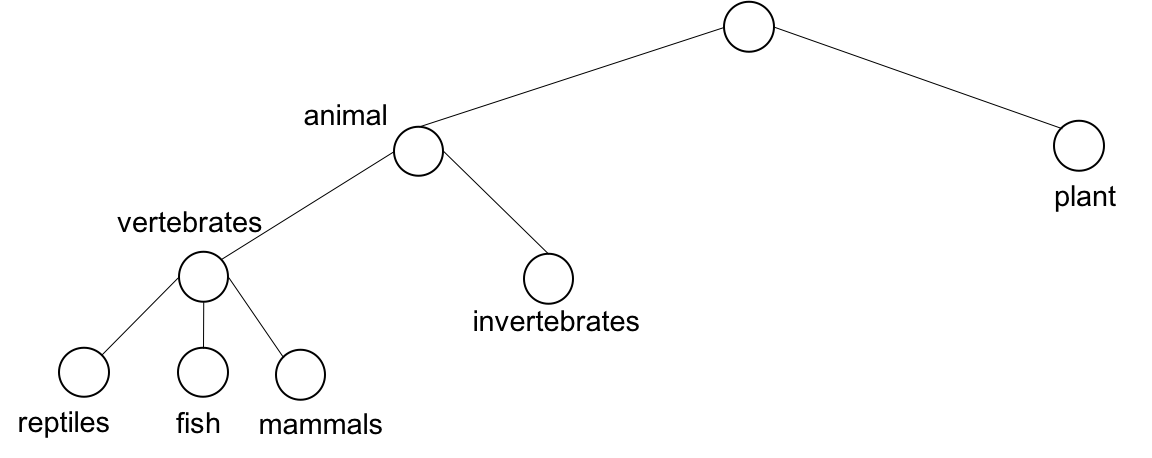
\includegraphics[width=0.7\textwidth]{cifar100_after.png}
%   \fbox{\rule[-.5cm]{0cm}{4cm}{fig1.jpg} \rule[-.5cm]{4cm}{0cm}}
  \caption{Output taxonomy-based tree}
\end{figure}

\begin{table}[t]
  \caption{Accuracy of each node}
  \label{sample-table}
  \centering
  \begin{tabular}{lll}
    \toprule
    % \multicolumn{2}{c}{Part}                   \\
    \cmidrule{1-2}
    Name     & \# of samples & Accuracy \\
    \midrule
    animal & 17500 & 71\% \\
    vertebrates & 12500 & 60\% \\
    reptiles+fish & 5000 & 10\% \\
    mammals & 7500 & 6\% \\
    invertebrates & 5000 & 50\% \\
    insects & 2500 & 20\% \\
    otherinverts. & 2500 & 20\% \\
    people & 2000 & 50\% \\ 
    plant & 7500 & 6\% \\ 
    root node & 27000 & 65\% \\
    \bottomrule
  \end{tabular}
\end{table}

\section{Timeline and Division of Work }
We have mainly met our goal set in the project proposal.\\
4/16-4/22:\\
Run NNs on Raspberry Pis. Profile the Raspberry Pis for maximum size of networks and communication overhead (hfang). Find better clustering methods/pruning decisions.(hfang,jzuo,yichenr)\\
4/23-4/29:\\
Implement maximum NNs on Raspberry Pis. Tune the hyperparameters of the current structure for higher accuracy. (jzuo,yichenr) Fix upon a final design and gather data for poster/demo. (hfang)



\newpage
\section*{References}

\medskip

\small

[1] https://cloud.google.com/solutions/automating-iot-machine-learning.

[2] https://docs.microsoft.com/en-us/azure/iot-edge/tutorial-deploy-machine-learning.

[3] https://microsoft.github.io/ELL/.

[4] Kumar, A., Goyal, S. \& Varma, M. (2017). Resource-efficient Machine Learning in 2 KB RAM for the Internet of Things. In {\it International Conference on Machine Learning}, pp. 1935-1944.

[5] Li, M., Andersen, D. G., Smola, A. J., \& Yu, K. (2014). Communication efficient distributed machine learning with the parameter server. In {\it Advances in Neural Information Processing Systems}, pp. 19-27.

[6] Hsieh, K., Harlap, A., Vijaykumar, N., Konomis, D., Ganger, G. R., Gibbons, P. B., \& Mutlu, O. (2017). Gaia: Geo-Distributed Machine Learning Approaching LAN Speeds. In {\it NSDI}, pp. 629-647.

[7] Cui, H., Zhang, H., Ganger, G. R., Gibbons, P. B., \& Xing, E. P. (2016). GeePS: Scalable deep learning on distributed GPUs with a GPU-specialized parameter server. In {\it Proceedings of the Eleventh European Conference on Computer Systems}.

[8] Xing, E. P., Ho, Q., Dai, W., Kim, J.K., Wei, J., Lee, S., Zheng, X., Xie, P., Kumar, A. \& Yu, Y. (2015). Petuum: A new platform for distributed machine learning on big data. {\it IEEE Transactions on Big Data}, 1(2), pp. 49-67.

[9] Trapeznikov, K., \& Saligrama, V. (2013). Supervised sequential classification under budget constraints. In {\it Artificial Intelligence and Statistics}, pp. 581-589.

[10] Xu, Z., Weinberger, K., \& Chapelle, O. (2012). The greedy miser: Learning under test-time budgets. In {\it Proceedings of the 29th International Conference on Machine Learning}.

[11] Nan, F. \& Saligrama, V. (2017). Adaptive Classification for Prediction Under a Budget. In {\it Advances in Neural Information Processing Systems}, pp. 4730-4740.

[12] Nan, F., Wang, J., \& Saligrama, V. (2016). Pruning random forests for prediction on a budget. In {\it Advances in neural information processing systems}, pp. 2334-2342.

[13] Gupta, C., Suggala, A.S., Goyal, A., Simhadri, H.V., Paranjape, B., Kumar, A., Goyal, S., Udupa, R., Varma, M. \& Jain, P. (2017). ProtoNN: Compressed and Accurate kNN for Resource-scarce Devices. In {\it International Conference on Machine Learning}, pp. 1331-1340.

[14] Garg, V. K., Dekel, O., \& Xiao, L. (2018). Learning SMaLL Predictors. arXiv preprint arXiv:1803.02388.


\end{document}
